% Options for packages loaded elsewhere
\PassOptionsToPackage{unicode}{hyperref}
\PassOptionsToPackage{hyphens}{url}
%
\documentclass[
]{article}
\usepackage{lmodern}
\usepackage{amssymb,amsmath}
\usepackage{ifxetex,ifluatex}
\ifnum 0\ifxetex 1\fi\ifluatex 1\fi=0 % if pdftex
  \usepackage[T1]{fontenc}
  \usepackage[utf8]{inputenc}
  \usepackage{textcomp} % provide euro and other symbols
\else % if luatex or xetex
  \usepackage{unicode-math}
  \defaultfontfeatures{Scale=MatchLowercase}
  \defaultfontfeatures[\rmfamily]{Ligatures=TeX,Scale=1}
\fi
% Use upquote if available, for straight quotes in verbatim environments
\IfFileExists{upquote.sty}{\usepackage{upquote}}{}
\IfFileExists{microtype.sty}{% use microtype if available
  \usepackage[]{microtype}
  \UseMicrotypeSet[protrusion]{basicmath} % disable protrusion for tt fonts
}{}
\makeatletter
\@ifundefined{KOMAClassName}{% if non-KOMA class
  \IfFileExists{parskip.sty}{%
    \usepackage{parskip}
  }{% else
    \setlength{\parindent}{0pt}
    \setlength{\parskip}{6pt plus 2pt minus 1pt}}
}{% if KOMA class
  \KOMAoptions{parskip=half}}
\makeatother
\usepackage{xcolor}
\IfFileExists{xurl.sty}{\usepackage{xurl}}{} % add URL line breaks if available
\IfFileExists{bookmark.sty}{\usepackage{bookmark}}{\usepackage{hyperref}}
\hypersetup{
  pdftitle={Running multiple analyses at once using the CohortMethod package},
  pdfauthor={Martijn J. Schuemie, Marc A. Suchard and Patrick Ryan},
  hidelinks,
  pdfcreator={LaTeX via pandoc}}
\urlstyle{same} % disable monospaced font for URLs
\usepackage[margin=1in]{geometry}
\usepackage{color}
\usepackage{fancyvrb}
\newcommand{\VerbBar}{|}
\newcommand{\VERB}{\Verb[commandchars=\\\{\}]}
\DefineVerbatimEnvironment{Highlighting}{Verbatim}{commandchars=\\\{\}}
% Add ',fontsize=\small' for more characters per line
\usepackage{framed}
\definecolor{shadecolor}{RGB}{248,248,248}
\newenvironment{Shaded}{\begin{snugshade}}{\end{snugshade}}
\newcommand{\AlertTok}[1]{\textcolor[rgb]{0.94,0.16,0.16}{#1}}
\newcommand{\AnnotationTok}[1]{\textcolor[rgb]{0.56,0.35,0.01}{\textbf{\textit{#1}}}}
\newcommand{\AttributeTok}[1]{\textcolor[rgb]{0.77,0.63,0.00}{#1}}
\newcommand{\BaseNTok}[1]{\textcolor[rgb]{0.00,0.00,0.81}{#1}}
\newcommand{\BuiltInTok}[1]{#1}
\newcommand{\CharTok}[1]{\textcolor[rgb]{0.31,0.60,0.02}{#1}}
\newcommand{\CommentTok}[1]{\textcolor[rgb]{0.56,0.35,0.01}{\textit{#1}}}
\newcommand{\CommentVarTok}[1]{\textcolor[rgb]{0.56,0.35,0.01}{\textbf{\textit{#1}}}}
\newcommand{\ConstantTok}[1]{\textcolor[rgb]{0.00,0.00,0.00}{#1}}
\newcommand{\ControlFlowTok}[1]{\textcolor[rgb]{0.13,0.29,0.53}{\textbf{#1}}}
\newcommand{\DataTypeTok}[1]{\textcolor[rgb]{0.13,0.29,0.53}{#1}}
\newcommand{\DecValTok}[1]{\textcolor[rgb]{0.00,0.00,0.81}{#1}}
\newcommand{\DocumentationTok}[1]{\textcolor[rgb]{0.56,0.35,0.01}{\textbf{\textit{#1}}}}
\newcommand{\ErrorTok}[1]{\textcolor[rgb]{0.64,0.00,0.00}{\textbf{#1}}}
\newcommand{\ExtensionTok}[1]{#1}
\newcommand{\FloatTok}[1]{\textcolor[rgb]{0.00,0.00,0.81}{#1}}
\newcommand{\FunctionTok}[1]{\textcolor[rgb]{0.00,0.00,0.00}{#1}}
\newcommand{\ImportTok}[1]{#1}
\newcommand{\InformationTok}[1]{\textcolor[rgb]{0.56,0.35,0.01}{\textbf{\textit{#1}}}}
\newcommand{\KeywordTok}[1]{\textcolor[rgb]{0.13,0.29,0.53}{\textbf{#1}}}
\newcommand{\NormalTok}[1]{#1}
\newcommand{\OperatorTok}[1]{\textcolor[rgb]{0.81,0.36,0.00}{\textbf{#1}}}
\newcommand{\OtherTok}[1]{\textcolor[rgb]{0.56,0.35,0.01}{#1}}
\newcommand{\PreprocessorTok}[1]{\textcolor[rgb]{0.56,0.35,0.01}{\textit{#1}}}
\newcommand{\RegionMarkerTok}[1]{#1}
\newcommand{\SpecialCharTok}[1]{\textcolor[rgb]{0.00,0.00,0.00}{#1}}
\newcommand{\SpecialStringTok}[1]{\textcolor[rgb]{0.31,0.60,0.02}{#1}}
\newcommand{\StringTok}[1]{\textcolor[rgb]{0.31,0.60,0.02}{#1}}
\newcommand{\VariableTok}[1]{\textcolor[rgb]{0.00,0.00,0.00}{#1}}
\newcommand{\VerbatimStringTok}[1]{\textcolor[rgb]{0.31,0.60,0.02}{#1}}
\newcommand{\WarningTok}[1]{\textcolor[rgb]{0.56,0.35,0.01}{\textbf{\textit{#1}}}}
\usepackage{graphicx,grffile}
\makeatletter
\def\maxwidth{\ifdim\Gin@nat@width>\linewidth\linewidth\else\Gin@nat@width\fi}
\def\maxheight{\ifdim\Gin@nat@height>\textheight\textheight\else\Gin@nat@height\fi}
\makeatother
% Scale images if necessary, so that they will not overflow the page
% margins by default, and it is still possible to overwrite the defaults
% using explicit options in \includegraphics[width, height, ...]{}
\setkeys{Gin}{width=\maxwidth,height=\maxheight,keepaspectratio}
% Set default figure placement to htbp
\makeatletter
\def\fps@figure{htbp}
\makeatother
\setlength{\emergencystretch}{3em} % prevent overfull lines
\providecommand{\tightlist}{%
  \setlength{\itemsep}{0pt}\setlength{\parskip}{0pt}}
\setcounter{secnumdepth}{5}

\title{Running multiple analyses at once using the CohortMethod package}
\author{Martijn J. Schuemie, Marc A. Suchard and Patrick Ryan}
\date{2020-05-19}

\begin{document}
\maketitle

{
\setcounter{tocdepth}{2}
\tableofcontents
}
\hypertarget{introduction}{%
\section{Introduction}\label{introduction}}

In this vignette we focus on running several different analyses on
several target-comparator-outcome combinations. This can be useful when
we want to explore the sensitivity to analyses choices, include
controls, or run an experiment similar to the OMOP experiment to
empirically identify the optimal analysis choices for a particular
research question.

This vignette assumes you are already familiar with the
\texttt{CohortMethod} package and are able to perform single studies. We
will walk through all the steps needed to perform an exemplar set of
analyses, and we have selected the well-studied topic of the effect of
coxibs versus non-selective nonsteroidal anti-inflammatory drugs
(NSAIDs) on gastrointestinal (GI) bleeding-related hospitalization. For
simplicity, we focus on one coxib -- celecoxib -- and one non-selective
NSAID -- diclofenac. We will execute various variations of an analysis
for the primary outcome and a large set of negative control outcomes.

\hypertarget{general-approach}{%
\section{General approach}\label{general-approach}}

The general approach to running a set of analyses is that you specify
all the function arguments of the functions you would normally call, and
create sets of these function arguments. The final outcome models as
well as intermediate data objects will all be saved to disk for later
extraction.

An analysis will be executed by calling these functions in sequence:

\begin{enumerate}
\def\labelenumi{\arabic{enumi}.}
\tightlist
\item
  \texttt{getDbCohortMethodData()}
\item
  \texttt{createStudyPopulation()}
\item
  \texttt{createPs()} (optional)
\item
  \texttt{trimByPs()} or \texttt{trimByPsToEquipoise()} (optional)
\item
  \texttt{matchOnPs()}, \texttt{matchOnPsAndCovariates()},
  \texttt{stratifyByPs()}, or \texttt{stratifyByPsAndCovariates()}
  (optional)
\item
  \texttt{fitOutcomeModel()} (optional)
\end{enumerate}

When you provide several analyses to the \texttt{CohortMethod} package,
it will determine whether any of the analyses have anything in common,
and will take advantage of this fact. For example, if we specify several
analyses that only differ in the way the outcome model is fitted, then
\texttt{CohortMethod} will extract the data and fit the propensity model
only once, and re-use this in all the analyses.

The function arguments you need to define have been divided into four
groups:

\begin{enumerate}
\def\labelenumi{\arabic{enumi}.}
\tightlist
\item
  \textbf{Hypothesis of interest}: arguments that are specific to a
  hypothesis of interest, in the case of the cohort method this is a
  combination of target, comparator, and outcome.
\item
  \textbf{Analyses}: arguments that are not directly specific to a
  hypothesis of interest, such as the washout window, whether to include
  drugs as covariates, etc.
\item
  Arguments that are the output of a previous function in the
  \texttt{CohortMethod} package, such as the \texttt{cohortMethodData}
  argument of the \texttt{createPs} function. These cannot be specified
  by the user.
\item
  Arguments that are specific to an environment, such as the connection
  details for connecting to the server, and the name of the schema
  holding the CDM data.
\end{enumerate}

There are a two arguments (\texttt{excludedCovariateConceptIds}, and
\texttt{includedCovariateConceptIds} of the
\texttt{getDbCohortMethodData()} function) that can be argued to be part
both of group 1 and 2. These arguments are therefore present in both
groups, and when executing the analysis the union of the two lists of
concept IDs will be used.

\hypertarget{preparation-for-the-example}{%
\section{Preparation for the
example}\label{preparation-for-the-example}}

We need to tell R how to connect to the server where the data are.
\texttt{CohortMethod} uses the \texttt{DatabaseConnector} package, which
provides the \texttt{createConnectionDetails} function. Type
\texttt{?createConnectionDetails} for the specific settings required for
the various database management systems (DBMS). For example, one might
connect to a PostgreSQL database using this code:

\begin{Shaded}
\begin{Highlighting}[]
\NormalTok{connectionDetails <-}\StringTok{ }\KeywordTok{createConnectionDetails}\NormalTok{(}\DataTypeTok{dbms =} \StringTok{"postgresql"}\NormalTok{, }
                                             \DataTypeTok{server =} \StringTok{"localhost/ohdsi"}\NormalTok{, }
                                             \DataTypeTok{user =} \StringTok{"joe"}\NormalTok{, }
                                             \DataTypeTok{password =} \StringTok{"supersecret"}\NormalTok{)}

\NormalTok{cdmDatabaseSchema <-}\StringTok{ "my_cdm_data"}
\NormalTok{resultsDatabaseSchema <-}\StringTok{ "my_results"}
\NormalTok{outputFolder <-}\StringTok{ "./CohortMethodOutput"}
\end{Highlighting}
\end{Shaded}

The last three lines define the \texttt{cdmDatabaseSchema},
\texttt{resultSchema}, and \texttt{outputFolder} variables. We'll use
these later to tell R where the data in CDM format live, where we want
to write intermediate tables, and where the intermediate and output
files should be stored in the local file system. Note that for Microsoft
SQL Server, databaseschemas need to specify both the database and the
schema, so for example
\texttt{cdmDatabaseSchema\ \textless{}-\ "my\_cdm\_data.dbo"}.

We also need to prepare our exposures and outcomes of interest. The
drug\_era table in the OMOP Common Data Model already contains
prespecified cohorts of users at the ingredient level, so we will use
that for the exposures. For the outcomes, we want to restrict our
analysis only to those outcomes that are recorded in an inpatient
setting, so we will need to create a custom cohort table. For this
example, we want to include GI bleed (concept ID 192671) as well as a
set of 35 negative controls. Negative controls are defined as those
outcomes where there is no evidence that either the target drug
(celexocib) or comparator drug (diclofenac) causes the outcome.

We create a text file called \emph{VignetteOutcomes.sql} with the
following content:

\begin{Shaded}
\begin{Highlighting}[]
\CommentTok{/***********************************}
\CommentTok{File VignetteOutcomes.sql}
\CommentTok{***********************************/}
\ControlFlowTok{IF}\NormalTok{ OBJECT_ID(}\StringTok{'@resultsDatabaseSchema.outcomes'}\NormalTok{, }\StringTok{'U'}\NormalTok{) }\KeywordTok{IS} \KeywordTok{NOT} \KeywordTok{NULL}
  \KeywordTok{DROP} \KeywordTok{TABLE}\NormalTok{ @resultsDatabaseSchema.outcomes;}

\KeywordTok{SELECT}\NormalTok{ ancestor_concept_id }\KeywordTok{AS}\NormalTok{ cohort_definition_id,}
\NormalTok{    condition_start_date }\KeywordTok{AS}\NormalTok{ cohort_start_date,}
\NormalTok{    condition_end_date }\KeywordTok{AS}\NormalTok{ cohort_end_date,}
\NormalTok{    condition_occurrence.person_id }\KeywordTok{AS}\NormalTok{ subject_id}
\KeywordTok{INTO}\NormalTok{ @resultsDatabaseSchema.outcomes}
\KeywordTok{FROM}\NormalTok{ @cdmDatabaseSchema.condition_occurrence}
\KeywordTok{INNER} \KeywordTok{JOIN}\NormalTok{ @cdmDatabaseSchema.visit_occurrence}
    \KeywordTok{ON}\NormalTok{ condition_occurrence.visit_occurrence_id }\OperatorTok{=}\NormalTok{ visit_occurrence.visit_occurrence_id}
\KeywordTok{INNER} \KeywordTok{JOIN}\NormalTok{ @cdmDatabaseSchema.concept_ancestor}
    \KeywordTok{ON}\NormalTok{ condition_concept_id }\OperatorTok{=}\NormalTok{ descendant_concept_id}
\KeywordTok{WHERE}\NormalTok{ ancestor_concept_id }\KeywordTok{IN}\NormalTok{ (}\DecValTok{192671}\NormalTok{, }\DecValTok{24609}\NormalTok{, }\DecValTok{29735}\NormalTok{, }\DecValTok{73754}\NormalTok{, }\DecValTok{80004}\NormalTok{, }\DecValTok{134718}\NormalTok{, }\DecValTok{139099}\NormalTok{,}
\DecValTok{141932}\NormalTok{, }\DecValTok{192367}\NormalTok{, }\DecValTok{193739}\NormalTok{, }\DecValTok{194997}\NormalTok{, }\DecValTok{197236}\NormalTok{, }\DecValTok{199074}\NormalTok{, }\DecValTok{255573}\NormalTok{, }\DecValTok{257007}\NormalTok{, }\DecValTok{313459}\NormalTok{, }\DecValTok{314658}\NormalTok{,}
\DecValTok{316084}\NormalTok{, }\DecValTok{319843}\NormalTok{, }\DecValTok{321596}\NormalTok{, }\DecValTok{374366}\NormalTok{, }\DecValTok{375292}\NormalTok{, }\DecValTok{380094}\NormalTok{, }\DecValTok{433753}\NormalTok{, }\DecValTok{433811}\NormalTok{, }\DecValTok{436665}\NormalTok{, }\DecValTok{436676}\NormalTok{,}
\DecValTok{436940}\NormalTok{, }\DecValTok{437784}\NormalTok{, }\DecValTok{438134}\NormalTok{, }\DecValTok{440358}\NormalTok{, }\DecValTok{440374}\NormalTok{, }\DecValTok{443617}\NormalTok{, }\DecValTok{443800}\NormalTok{, }\DecValTok{4084966}\NormalTok{, }\DecValTok{4288310}\NormalTok{)}
    \KeywordTok{AND}\NormalTok{ visit_occurrence.visit_concept_id }\KeywordTok{IN}\NormalTok{ (}\DecValTok{9201}\NormalTok{, }\DecValTok{9203}\NormalTok{);}
\end{Highlighting}
\end{Shaded}

This is parameterized SQL which can be used by the \texttt{SqlRender}
package. We use parameterized SQL so we do not have to pre-specify the
names of the CDM and result schemas. That way, if we want to run the SQL
on a different schema, we only need to change the parameter values; we
do not have to change the SQL code. By also making use of translation
functionality in \texttt{SqlRender}, we can make sure the SQL code can
be run in many different environments.

\begin{Shaded}
\begin{Highlighting}[]
\KeywordTok{library}\NormalTok{(SqlRender)}
\NormalTok{sql <-}\StringTok{ }\KeywordTok{readSql}\NormalTok{(}\StringTok{"VignetteOutcomes.sql"}\NormalTok{)}
\NormalTok{sql <-}\StringTok{ }\KeywordTok{render}\NormalTok{(sql,}
              \DataTypeTok{cdmDatabaseSchema =}\NormalTok{ cdmDatabaseSchema, }
              \DataTypeTok{resultsDatabaseSchema =}\NormalTok{ resultsDatabaseSchema)}
\NormalTok{sql <-}\StringTok{ }\KeywordTok{translate}\NormalTok{(sql, }\DataTypeTok{targetDialect =}\NormalTok{ connectionDetails}\OperatorTok{$}\NormalTok{dbms)}

\NormalTok{connection <-}\StringTok{ }\KeywordTok{connect}\NormalTok{(connectionDetails)}
\KeywordTok{executeSql}\NormalTok{(connection, sql)}
\end{Highlighting}
\end{Shaded}

In this code, we first read the SQL from the file into memory. In the
next line, we replace the two parameter names with the actual values. We
then translate the SQL into the dialect appropriate for the DBMS we
already specified in the \texttt{connectionDetails}. Next, we connect to
the server, and submit the rendered and translated SQL.

\hypertarget{specifying-hypotheses-of-interest}{%
\section{Specifying hypotheses of
interest}\label{specifying-hypotheses-of-interest}}

The first group of arguments define the target, comparator, and outcome.
Here we demonstrate how to create one set, and add that set to a list:

\begin{Shaded}
\begin{Highlighting}[]
\NormalTok{tcos <-}\StringTok{ }\KeywordTok{createTargetComparatorOutcomes}\NormalTok{(}\DataTypeTok{targetId =} \DecValTok{1118084}\NormalTok{,}
                                       \DataTypeTok{comparatorId =} \DecValTok{1124300}\NormalTok{,}
                                       \DataTypeTok{outcomeIds =} \KeywordTok{c}\NormalTok{(}\DecValTok{192671}\NormalTok{, }\DecValTok{29735}\NormalTok{, }\DecValTok{140673}\NormalTok{, }\DecValTok{197494}\NormalTok{, }
                                                      \DecValTok{198185}\NormalTok{, }\DecValTok{198199}\NormalTok{, }\DecValTok{200528}\NormalTok{, }\DecValTok{257315}\NormalTok{, }
                                                      \DecValTok{314658}\NormalTok{, }\DecValTok{317376}\NormalTok{, }\DecValTok{321319}\NormalTok{, }\DecValTok{380731}\NormalTok{, }
                                                      \DecValTok{432661}\NormalTok{, }\DecValTok{432867}\NormalTok{, }\DecValTok{433516}\NormalTok{, }\DecValTok{433701}\NormalTok{, }
                                                      \DecValTok{433753}\NormalTok{, }\DecValTok{435140}\NormalTok{, }\DecValTok{435459}\NormalTok{, }\DecValTok{435524}\NormalTok{, }
                                                      \DecValTok{435783}\NormalTok{, }\DecValTok{436665}\NormalTok{, }\DecValTok{436676}\NormalTok{, }\DecValTok{442619}\NormalTok{, }
                                                      \DecValTok{444252}\NormalTok{, }\DecValTok{444429}\NormalTok{, }\DecValTok{4131756}\NormalTok{, }\DecValTok{4134120}\NormalTok{, }
                                                      \DecValTok{4134454}\NormalTok{, }\DecValTok{4152280}\NormalTok{, }\DecValTok{4165112}\NormalTok{, }\DecValTok{4174262}\NormalTok{, }
                                                      \DecValTok{4182210}\NormalTok{, }\DecValTok{4270490}\NormalTok{, }\DecValTok{4286201}\NormalTok{, }\DecValTok{4289933}\NormalTok{))}

\NormalTok{targetComparatorOutcomesList <-}\StringTok{ }\KeywordTok{list}\NormalTok{(tcos)}
\end{Highlighting}
\end{Shaded}

We defined the target to be celecoxib (concept ID 1118084), the
comparator to be diclofenac (concept ID 1124300), and the outcomes of
interest are GI-bleed (concept ID 192671) and a large number of negative
control outcomes.

A convenient way to save \texttt{targetComparatorOutcomesList} to file
is by using the \texttt{saveTargetComparatorOutcomesList} function, and
we can load it again using the \texttt{loadTargetComparatorOutcomesList}
function.

\hypertarget{specifying-analyses}{%
\section{Specifying analyses}\label{specifying-analyses}}

The second group of arguments are not specific to a hypothesis of
interest, and comprise the majority of arguments. For each function that
will be called during the execution of the analyses, a companion
function is available that has (almost) the same arguments. For example,
for the \texttt{trimByPs()} function there is the
\texttt{createTrimByPsArgs()} function. These companion functions can be
used to create the arguments to be used during execution:

\begin{Shaded}
\begin{Highlighting}[]
\NormalTok{nsaids <-}\StringTok{ }\DecValTok{21603933}

\NormalTok{covarSettings <-}\StringTok{ }\KeywordTok{createDefaultCovariateSettings}\NormalTok{(}\DataTypeTok{excludedCovariateConceptIds =}\NormalTok{ nsaids,}
                                                \DataTypeTok{addDescendantsToExclude =} \OtherTok{TRUE}\NormalTok{)}

\NormalTok{getDbCmDataArgs <-}\StringTok{ }\KeywordTok{createGetDbCohortMethodDataArgs}\NormalTok{(}\DataTypeTok{washoutPeriod =} \DecValTok{183}\NormalTok{,}
                                                   \DataTypeTok{restrictToCommonPeriod =} \OtherTok{FALSE}\NormalTok{,}
                                                   \DataTypeTok{firstExposureOnly =} \OtherTok{TRUE}\NormalTok{,}
                                                   \DataTypeTok{removeDuplicateSubjects =} \StringTok{"remove all"}\NormalTok{,}
                                                   \DataTypeTok{studyStartDate =} \StringTok{""}\NormalTok{,}
                                                   \DataTypeTok{studyEndDate =} \StringTok{""}\NormalTok{,}
                                                   \DataTypeTok{excludeDrugsFromCovariates =} \OtherTok{FALSE}\NormalTok{,}
                                                   \DataTypeTok{covariateSettings =}\NormalTok{ covarSettings)}

\NormalTok{createStudyPopArgs <-}\StringTok{ }\KeywordTok{createCreateStudyPopulationArgs}\NormalTok{(}\DataTypeTok{removeSubjectsWithPriorOutcome =} \OtherTok{TRUE}\NormalTok{,}
                                                      \DataTypeTok{minDaysAtRisk =} \DecValTok{1}\NormalTok{,}
                                                      \DataTypeTok{riskWindowStart =} \DecValTok{0}\NormalTok{,}
                                                      \DataTypeTok{startAnchor =} \StringTok{"cohort start"}\NormalTok{,}
                                                      \DataTypeTok{riskWindowEnd =} \DecValTok{30}\NormalTok{,}
                                                      \DataTypeTok{endAnchor =} \StringTok{"cohort end"}\NormalTok{)}

\NormalTok{fitOutcomeModelArgs1 <-}\StringTok{ }\KeywordTok{createFitOutcomeModelArgs}\NormalTok{(}\DataTypeTok{modelType =} \StringTok{"cox"}\NormalTok{)}
\end{Highlighting}
\end{Shaded}

Any argument that is not explicitly specified by the user will assume
the default value specified in the function. We can now combine the
arguments for the various functions into a single analysis:

\begin{Shaded}
\begin{Highlighting}[]
\NormalTok{cmAnalysis1 <-}\StringTok{ }\KeywordTok{createCmAnalysis}\NormalTok{(}\DataTypeTok{analysisId =} \DecValTok{1}\NormalTok{,}
                                \DataTypeTok{description =} \StringTok{"No matching, simple outcome model"}\NormalTok{,}
                                \DataTypeTok{getDbCohortMethodDataArgs =}\NormalTok{ getDbCmDataArgs,}
                                \DataTypeTok{createStudyPopArgs =}\NormalTok{ createStudyPopArgs,}
                                \DataTypeTok{fitOutcomeModel =} \OtherTok{TRUE}\NormalTok{,}
                                \DataTypeTok{fitOutcomeModelArgs =}\NormalTok{ fitOutcomeModelArgs1)}
\end{Highlighting}
\end{Shaded}

Note that we have assigned an analysis ID (1) to this set of arguments.
We can use this later to link the results back to this specific set of
choices. We also include a short description of the analysis.

We can easily create more analyses, for example by using matching,
stratification, inverse probability of treatment weighting, or by using
more sophisticated outcome models:

\begin{Shaded}
\begin{Highlighting}[]
\NormalTok{createPsArgs <-}\StringTok{ }\KeywordTok{createCreatePsArgs}\NormalTok{() }\CommentTok{# Use default settings only}

\NormalTok{matchOnPsArgs <-}\StringTok{ }\KeywordTok{createMatchOnPsArgs}\NormalTok{(}\DataTypeTok{maxRatio =} \DecValTok{100}\NormalTok{)}

\NormalTok{fitOutcomeModelArgs2 <-}\StringTok{ }\KeywordTok{createFitOutcomeModelArgs}\NormalTok{(}\DataTypeTok{modelType =} \StringTok{"cox"}\NormalTok{,}
                                                  \DataTypeTok{stratified =} \OtherTok{TRUE}\NormalTok{)}

\NormalTok{cmAnalysis2 <-}\StringTok{ }\KeywordTok{createCmAnalysis}\NormalTok{(}\DataTypeTok{analysisId =} \DecValTok{2}\NormalTok{,}
                                \DataTypeTok{description =} \StringTok{"Matching"}\NormalTok{,}
                                \DataTypeTok{getDbCohortMethodDataArgs =}\NormalTok{ getDbCmDataArgs,}
                                \DataTypeTok{createStudyPopArgs =}\NormalTok{ createStudyPopArgs,}
                                \DataTypeTok{createPs =} \OtherTok{TRUE}\NormalTok{,}
                                \DataTypeTok{createPsArgs =}\NormalTok{ createPsArgs,}
                                \DataTypeTok{matchOnPs =} \OtherTok{TRUE}\NormalTok{,}
                                \DataTypeTok{matchOnPsArgs =}\NormalTok{ matchOnPsArgs,}
                                \DataTypeTok{fitOutcomeModel =} \OtherTok{TRUE}\NormalTok{,}
                                \DataTypeTok{fitOutcomeModelArgs =}\NormalTok{ fitOutcomeModelArgs1)}

\NormalTok{stratifyByPsArgs <-}\StringTok{ }\KeywordTok{createStratifyByPsArgs}\NormalTok{(}\DataTypeTok{numberOfStrata =} \DecValTok{5}\NormalTok{)}

\NormalTok{cmAnalysis3 <-}\StringTok{ }\KeywordTok{createCmAnalysis}\NormalTok{(}\DataTypeTok{analysisId =} \DecValTok{3}\NormalTok{,}
                                \DataTypeTok{description =} \StringTok{"Stratification"}\NormalTok{,}
                                \DataTypeTok{getDbCohortMethodDataArgs =}\NormalTok{ getDbCmDataArgs,}
                                \DataTypeTok{createStudyPopArgs =}\NormalTok{ createStudyPopArgs,}
                                \DataTypeTok{createPs =} \OtherTok{TRUE}\NormalTok{,}
                                \DataTypeTok{createPsArgs =}\NormalTok{ createPsArgs,}
                                \DataTypeTok{stratifyByPs =} \OtherTok{TRUE}\NormalTok{,}
                                \DataTypeTok{stratifyByPsArgs =}\NormalTok{ stratifyByPsArgs,}
                                \DataTypeTok{fitOutcomeModel =} \OtherTok{TRUE}\NormalTok{,}
                                \DataTypeTok{fitOutcomeModelArgs =}\NormalTok{ fitOutcomeModelArgs2)}

\NormalTok{fitOutcomeModelArgs3 <-}\StringTok{ }\KeywordTok{createFitOutcomeModelArgs}\NormalTok{(}\DataTypeTok{modelType =} \StringTok{"cox"}\NormalTok{,}
                                                  \DataTypeTok{inversePtWeighting =} \OtherTok{TRUE}\NormalTok{)}

\NormalTok{cmAnalysis4 <-}\StringTok{ }\KeywordTok{createCmAnalysis}\NormalTok{(}\DataTypeTok{analysisId =} \DecValTok{4}\NormalTok{,}
                                \DataTypeTok{description =} \StringTok{"Inverse probability weighting"}\NormalTok{,}
                                \DataTypeTok{getDbCohortMethodDataArgs =}\NormalTok{ getDbCmDataArgs,}
                                \DataTypeTok{createStudyPopArgs =}\NormalTok{ createStudyPopArgs,}
                                \DataTypeTok{createPs =} \OtherTok{TRUE}\NormalTok{,}
                                \DataTypeTok{createPsArgs =}\NormalTok{ createPsArgs,}
                                \DataTypeTok{fitOutcomeModel =} \OtherTok{TRUE}\NormalTok{,}
                                \DataTypeTok{fitOutcomeModelArgs =}\NormalTok{ fitOutcomeModelArgs3)}

\NormalTok{fitOutcomeModelArgs4 <-}\StringTok{ }\KeywordTok{createFitOutcomeModelArgs}\NormalTok{(}\DataTypeTok{useCovariates =} \OtherTok{TRUE}\NormalTok{,}
                                                  \DataTypeTok{modelType =} \StringTok{"cox"}\NormalTok{,}
                                                  \DataTypeTok{stratified =} \OtherTok{TRUE}\NormalTok{)}

\NormalTok{cmAnalysis5 <-}\StringTok{ }\KeywordTok{createCmAnalysis}\NormalTok{(}\DataTypeTok{analysisId =} \DecValTok{5}\NormalTok{,}
                                \DataTypeTok{description =} \StringTok{"Matching plus full outcome model"}\NormalTok{,}
                                \DataTypeTok{getDbCohortMethodDataArgs =}\NormalTok{ getDbCmDataArgs,}
                                \DataTypeTok{createStudyPopArgs =}\NormalTok{ createStudyPopArgs,}
                                \DataTypeTok{createPs =} \OtherTok{TRUE}\NormalTok{,}
                                \DataTypeTok{createPsArgs =}\NormalTok{ createPsArgs,}
                                \DataTypeTok{matchOnPs =} \OtherTok{TRUE}\NormalTok{,}
                                \DataTypeTok{matchOnPsArgs =}\NormalTok{ matchOnPsArgs,}
                                \DataTypeTok{fitOutcomeModel =} \OtherTok{TRUE}\NormalTok{,}
                                \DataTypeTok{fitOutcomeModelArgs =}\NormalTok{ fitOutcomeModelArgs4)}

\NormalTok{interactionCovariateIds <-}\StringTok{ }\KeywordTok{c}\NormalTok{(}\DecValTok{8532001}\NormalTok{, }\DecValTok{201826210}\NormalTok{, }\DecValTok{21600960413}\NormalTok{) }\CommentTok{# Female, T2DM, concurent use of antithrombotic agents}

\NormalTok{fitOutcomeModelArgs5 <-}\StringTok{ }\KeywordTok{createFitOutcomeModelArgs}\NormalTok{(}\DataTypeTok{modelType =} \StringTok{"cox"}\NormalTok{,}
                                                  \DataTypeTok{stratified =} \OtherTok{TRUE}\NormalTok{,}
                                                  \DataTypeTok{interactionCovariateIds =}\NormalTok{ interactionCovariateIds)}

\NormalTok{cmAnalysis6 <-}\StringTok{ }\KeywordTok{createCmAnalysis}\NormalTok{(}\DataTypeTok{analysisId =} \DecValTok{6}\NormalTok{,}
                                \DataTypeTok{description =} \StringTok{"Stratification plus interaction terms"}\NormalTok{,}
                                \DataTypeTok{getDbCohortMethodDataArgs =}\NormalTok{ getDbCmDataArgs,}
                                \DataTypeTok{createStudyPopArgs =}\NormalTok{ createStudyPopArgs,}
                                \DataTypeTok{createPs =} \OtherTok{TRUE}\NormalTok{,}
                                \DataTypeTok{createPsArgs =}\NormalTok{ createPsArgs,}
                                \DataTypeTok{stratifyByPs =} \OtherTok{TRUE}\NormalTok{,}
                                \DataTypeTok{stratifyByPsArgs =}\NormalTok{ stratifyByPsArgs,}
                                \DataTypeTok{fitOutcomeModel =} \OtherTok{TRUE}\NormalTok{,}
                                \DataTypeTok{fitOutcomeModelArgs =}\NormalTok{ fitOutcomeModelArgs5)}
\end{Highlighting}
\end{Shaded}

These analyses can be combined in a list:

\begin{Shaded}
\begin{Highlighting}[]
\NormalTok{cmAnalysisList <-}\StringTok{ }\KeywordTok{list}\NormalTok{(cmAnalysis1, }
\NormalTok{                       cmAnalysis2, }
\NormalTok{                       cmAnalysis3, }
\NormalTok{                       cmAnalysis4, }
\NormalTok{                       cmAnalysis5, }
\NormalTok{                       cmAnalysis6)}
\end{Highlighting}
\end{Shaded}

A convenient way to save \texttt{cmAnalysisList} to file is by using the
\texttt{saveCmAnalysisList} function, and we can load it again using the
\texttt{loadCmAnalysisList} function.

\hypertarget{target-and-comparator-selection-strategies}{%
\subsection{Target and comparator selection
strategies}\label{target-and-comparator-selection-strategies}}

Often a new-user cohort design is used for comparative effectiveness
studies, where the selection of the comparator is part of the hypothesis
of interest: `Does use of drug A lead to an increased risk compared to
use of drug B?', where B is the comparator. But sometimes, the design is
used for safety assessment: `Does use of drug A lead to an increased
risk?' In this case the comparator is a proxy for the counterfactual of
no treatment. For example, we could pick the comparator to be a drug
known not to cause the outcome. we can argue that the selection of the
comparator then becomes part of the analyses specification, not the
hypothesis of interest, and we can have different strategies for
selecting a comparator: Do we for instance pick a drug in the same
class, or a drug with the same indication?

In the situation where the comparator choice becomes part of the
analyses, we can specify multiple comparators per hypothesis of interest
by using a list:

\begin{Shaded}
\begin{Highlighting}[]
\NormalTok{comparatorIds =}\StringTok{ }\KeywordTok{list}\NormalTok{(}\DataTypeTok{drugInSameClass =} \DecValTok{1124300}\NormalTok{,}
                     \DataTypeTok{drugWithSameIndication =} \DecValTok{1125315}\NormalTok{)}

\NormalTok{tcos <-}\StringTok{ }\KeywordTok{createTargetComparatorOutcomes}\NormalTok{(}\DataTypeTok{targetId =} \DecValTok{1118084}\NormalTok{,}
                                     \DataTypeTok{comparatorId =}\NormalTok{ comparatorIds,}
                                     \DataTypeTok{outcomeIds =} \DecValTok{192671}\NormalTok{)}

\NormalTok{targetComparatorOutcomesList2 <-}\StringTok{ }\KeywordTok{list}\NormalTok{(tcos)}
\end{Highlighting}
\end{Shaded}

When we specify an analysis, we can then refer to one comparator or
another:

\begin{Shaded}
\begin{Highlighting}[]
\NormalTok{cmAnalysis1 <-}\StringTok{ }\KeywordTok{createCmAnalysis}\NormalTok{(}\DataTypeTok{analysisId =} \DecValTok{1}\NormalTok{,}
                                \DataTypeTok{description =} \StringTok{"Analysis using drug in same class"}\NormalTok{,}
                                \DataTypeTok{comparatorType =} \StringTok{"drugInSameClass"}\NormalTok{,}
                                \DataTypeTok{getDbCohortMethodDataArgs =}\NormalTok{ getDbCmDataArgs,}
                                \DataTypeTok{createStudyPopArgs =}\NormalTok{ createStudyPopArgs,}
                                \DataTypeTok{createPs =} \OtherTok{TRUE}\NormalTok{,}
                                \DataTypeTok{createPsArgs =}\NormalTok{ createPsArgs,}
                                \DataTypeTok{matchOnPs =} \OtherTok{TRUE}\NormalTok{,}
                                \DataTypeTok{matchOnPsArgs =}\NormalTok{ matchOnPsArgs,}
                                \DataTypeTok{fitOutcomeModel =} \OtherTok{TRUE}\NormalTok{,}
                                \DataTypeTok{fitOutcomeModelArgs =}\NormalTok{ fitOutcomeModelArgs1)}

\NormalTok{cmAnalysis2 <-}\StringTok{ }\KeywordTok{createCmAnalysis}\NormalTok{(}\DataTypeTok{analysisId =} \DecValTok{2}\NormalTok{,}
                                \DataTypeTok{description =} \StringTok{"Analysis using drug with same indication"}\NormalTok{,}
                                \DataTypeTok{comparatorType =} \StringTok{"drugWithSameIndication"}\NormalTok{,}
                                \DataTypeTok{getDbCohortMethodDataArgs =}\NormalTok{ getDbCmDataArgs,}
                                \DataTypeTok{createStudyPopArgs =}\NormalTok{ createStudyPopArgs,}
                                \DataTypeTok{createPs =} \OtherTok{TRUE}\NormalTok{,}
                                \DataTypeTok{createPsArgs =}\NormalTok{ createPsArgs,}
                                \DataTypeTok{matchOnPs =} \OtherTok{TRUE}\NormalTok{,}
                                \DataTypeTok{matchOnPsArgs =}\NormalTok{ matchOnPsArgs,}
                                \DataTypeTok{fitOutcomeModel =} \OtherTok{TRUE}\NormalTok{,}
                                \DataTypeTok{fitOutcomeModelArgs =}\NormalTok{ fitOutcomeModelArgs1)}

\NormalTok{cmAnalysisList2 <-}\StringTok{ }\KeywordTok{list}\NormalTok{(cmAnalysis1, cmAnalysis2)}
\end{Highlighting}
\end{Shaded}

In this example, the first analysis (analysisID = 1) will use concept
1124300 as comparator, whilst the second analysis analysis (analysisID =
2) will use concept 1125315 as comparator.

The same mechanism can be used to specify types for the targetId.

\hypertarget{executing-multiple-analyses}{%
\section{Executing multiple
analyses}\label{executing-multiple-analyses}}

We can now run the analyses against the hypotheses of interest using the
\texttt{runCmAnalyses()} function. This function will run all specified
analyses against all hypotheses of interest, meaning that the total
number of outcome models is
\texttt{length(cmAnalysisList)\ *\ length(targetComparatorOutcomesList)}
(if all analyses specify an outcome model should be fitted).

\begin{Shaded}
\begin{Highlighting}[]
\NormalTok{result <-}\StringTok{ }\KeywordTok{runCmAnalyses}\NormalTok{(}\DataTypeTok{connectionDetails =}\NormalTok{ connectionDetails,}
                        \DataTypeTok{cdmDatabaseSchema =}\NormalTok{ cdmDatabaseSchema,}
                        \DataTypeTok{exposureDatabaseSchema =}\NormalTok{ cdmDatabaseSchema,}
                        \DataTypeTok{exposureTable =} \StringTok{"drug_era"}\NormalTok{,}
                        \DataTypeTok{outcomeDatabaseSchema =}\NormalTok{ resultsDatabaseSchema,}
                        \DataTypeTok{outcomeTable =} \StringTok{"outcomes"}\NormalTok{,}
                        \DataTypeTok{cdmVersion =}\NormalTok{ cdmVersion,}
                        \DataTypeTok{outputFolder =}\NormalTok{ outputFolder,}
                        \DataTypeTok{cmAnalysisList =}\NormalTok{ cmAnalysisList,}
                        \DataTypeTok{targetComparatorOutcomesList =}\NormalTok{ targetComparatorOutcomesList,}
                        \DataTypeTok{getDbCohortMethodDataThreads =} \DecValTok{1}\NormalTok{,}
                        \DataTypeTok{createPsThreads =} \DecValTok{1}\NormalTok{,}
                        \DataTypeTok{psCvThreads =} \DecValTok{10}\NormalTok{,}
                        \DataTypeTok{createStudyPopThreads =} \DecValTok{4}\NormalTok{,}
                        \DataTypeTok{trimMatchStratifyThreads =} \DecValTok{10}\NormalTok{,}
                        \DataTypeTok{fitOutcomeModelThreads =} \DecValTok{4}\NormalTok{,}
                        \DataTypeTok{outcomeCvThreads =} \DecValTok{10}\NormalTok{)}
\end{Highlighting}
\end{Shaded}

In the code above, we provide the arguments for connecting to the
database, which schemas and tables to use, as well as the analyses and
hypotheses of interest. The \texttt{outputFolder} specifies where the
outcome models and intermediate files will be written. We also instruct
\texttt{CohortMethod} to use multiple threads for various stages in the
analyses, meaning these will be executed in parallel on multiple CPUs in
the computer. Multithreading can significantly reduce execution time,
but will require more system resources such as memory and temporary disk
space.

\hypertarget{restarting}{%
\subsection{Restarting}\label{restarting}}

If for some reason the execution was interrupted, you can restart by
re-issuing the \texttt{runCmAnalyses()} command. Any intermediate and
final products that have already been completed and written to disk will
be skipped.

\hypertarget{retrieving-the-results}{%
\section{Retrieving the results}\label{retrieving-the-results}}

The result of the \texttt{runCmAnalyses()} is a data frame with one row
per target-target-outcome-analysis combination. It provides the file
names of the intermediate and end-result files that were constructed.
For example, we can retrieve and plot the propensity scores for the
combination of our target, comparator, outcome of interest, and last
analysis:

\begin{Shaded}
\begin{Highlighting}[]
\NormalTok{psFile <-}\StringTok{ }\NormalTok{result}\OperatorTok{$}\NormalTok{psFile[result}\OperatorTok{$}\NormalTok{targetId }\OperatorTok{==}\StringTok{ }\DecValTok{1118084} \OperatorTok{&}\StringTok{ }
\StringTok{                        }\NormalTok{result}\OperatorTok{$}\NormalTok{comparatorId }\OperatorTok{==}\StringTok{ }\DecValTok{1124300} \OperatorTok{&}\StringTok{ }
\StringTok{                        }\NormalTok{result}\OperatorTok{$}\NormalTok{outcomeId }\OperatorTok{==}\StringTok{ }\DecValTok{192671} \OperatorTok{&}
\StringTok{                        }\NormalTok{result}\OperatorTok{$}\NormalTok{analysisId }\OperatorTok{==}\StringTok{ }\DecValTok{5}\NormalTok{]}
\NormalTok{ps <-}\StringTok{ }\KeywordTok{readRDS}\NormalTok{(}\KeywordTok{file.path}\NormalTok{(outputFolder, psFile))}
\KeywordTok{plotPs}\NormalTok{(ps)}
\end{Highlighting}
\end{Shaded}

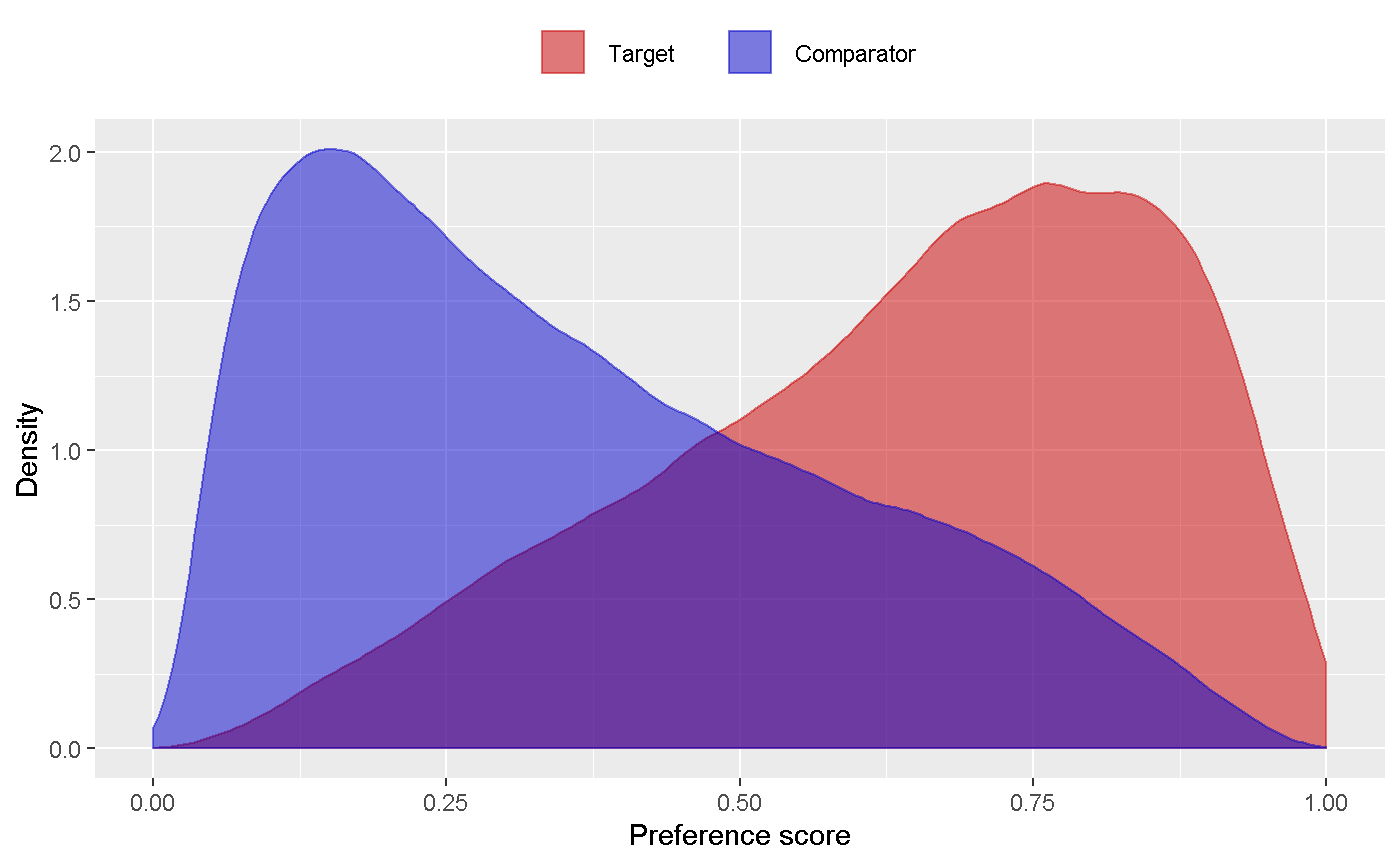
\includegraphics{../inst/doc/MultipleAnalyses_files/figure-latex/unnamed-chunk-13-1.pdf}

Note that some of the file names will appear several times in the table.
For example, analysis 3 and 5 only differ in terms of the outcome model,
and will share the same propensity score and stratification files.

We can create a summary of the results using
\texttt{summarizeAnalyses()}:

\begin{Shaded}
\begin{Highlighting}[]
\NormalTok{analysisSum <-}\StringTok{ }\KeywordTok{summarizeAnalyses}\NormalTok{(result, outputFolder)}
\KeywordTok{head}\NormalTok{(analysisSum)}
\end{Highlighting}
\end{Shaded}

\begin{verbatim}
## # A tibble: 6 x 31
##   analysisId targetId comparatorId outcomeId    rr ci95lb ci95ub        p target comparator targetDays comparatorDays eventsTarget eventsComparator  logRr seLogRr
##        <int>    <int>        <int>     <int> <dbl>  <dbl>  <dbl>    <dbl>  <int>      <int>      <dbl>          <dbl>        <dbl>            <dbl>  <dbl>   <dbl>
## 1          1  1118084      1124300     24609 1.33   0.954  1.86  9.63e- 2  62749      99138    8820539        7099392          106               61  0.283  0.170 
## 2          1  1118084      1124300     29735 1.49   1.05   2.13  2.77e- 2  62905      99332    8851773        7119415           87               55  0.397  0.181 
## 3          1  1118084      1124300     73754 1.25   0.895  1.75  1.93e- 1  62921      99322    8851724        7111142           92               65  0.223  0.171 
## 4          1  1118084      1124300     80004 0.548  0.487  0.615 4.89e-24  58760      90459    8227708        6492769          503              855 -0.602  0.0595
## 5          1  1118084      1124300    134718 3.63   0.550 71.2   2.99e- 1  63356      99899    8924706        7165598            5                1  1.29   1.24  
## 6          1  1118084      1124300    139099 0.715  0.394  1.28  2.66e- 1  63198      99600    8899286        7143451           22               28 -0.335  0.301 
## # ... with 15 more variables: rrI8532001 <dbl>, ci95lbI8532001 <dbl>, ci95ubI8532001 <dbl>, logRrI8532001 <dbl>, seLogRrI8532001 <dbl>, rrI201826210 <dbl>,
## #   ci95lbI201826210 <dbl>, ci95ubI201826210 <dbl>, logRrI201826210 <dbl>, seLogRrI201826210 <dbl>, rrI21600960413 <dbl>, ci95lbI21600960413 <dbl>,
## #   ci95ubI21600960413 <dbl>, logRrI21600960413 <dbl>, seLogRrI21600960413 <dbl>
\end{verbatim}

This tells us, per target-comparator-outcome-analysis combination, the
estimated relative risk and 95\% confidence interval, as well as the
number of people in the treated and comparator group (after trimming and
matching if applicable), and the number of outcomes observed for those
groups within the specified risk windows.

\hypertarget{empirical-calibration}{%
\subsection{Empirical calibration}\label{empirical-calibration}}

Now that we have produced estimates for all outcomes including our
negative controls, we can perform empirical calibration to estimate the
bias of the various analyses included in our study. We will create the
calibration effect plots for every analysis ID. In each plot, the blue
dots represent our negative control outcomes, and the yellow diamond
represents our health outcome of interest: GI bleed. An unbiased,
well-calibrated analysis should have 95\% of the negative controls
between the dashed lines (ie. 95\% should have p \textgreater{} .05).

\begin{Shaded}
\begin{Highlighting}[]
\KeywordTok{install.packages}\NormalTok{(}\StringTok{"EmpiricalCalibration"}\NormalTok{)}
\KeywordTok{library}\NormalTok{(EmpiricalCalibration)}

\CommentTok{# Analysis 1: No matching, simple outcome model}
\NormalTok{negCons <-}\StringTok{ }\NormalTok{analysisSum[analysisSum}\OperatorTok{$}\NormalTok{analysisId }\OperatorTok{==}\StringTok{ }\DecValTok{1} \OperatorTok{&}\StringTok{ }\NormalTok{analysisSum}\OperatorTok{$}\NormalTok{outcomeId }\OperatorTok{!=}\StringTok{ }\DecValTok{192671}\NormalTok{, ]}
\NormalTok{hoi <-}\StringTok{  }\NormalTok{analysisSum[analysisSum}\OperatorTok{$}\NormalTok{analysisId }\OperatorTok{==}\StringTok{ }\DecValTok{1} \OperatorTok{&}\StringTok{ }\NormalTok{analysisSum}\OperatorTok{$}\NormalTok{outcomeId }\OperatorTok{==}\StringTok{ }\DecValTok{192671}\NormalTok{, ]}
\NormalTok{null <-}\StringTok{ }\KeywordTok{fitNull}\NormalTok{(negCons}\OperatorTok{$}\NormalTok{logRr, negCons}\OperatorTok{$}\NormalTok{seLogRr)}
\KeywordTok{plotCalibrationEffect}\NormalTok{(negCons}\OperatorTok{$}\NormalTok{logRr, negCons}\OperatorTok{$}\NormalTok{seLogRr, hoi}\OperatorTok{$}\NormalTok{logRr, hoi}\OperatorTok{$}\NormalTok{seLogRr, null)}
\end{Highlighting}
\end{Shaded}

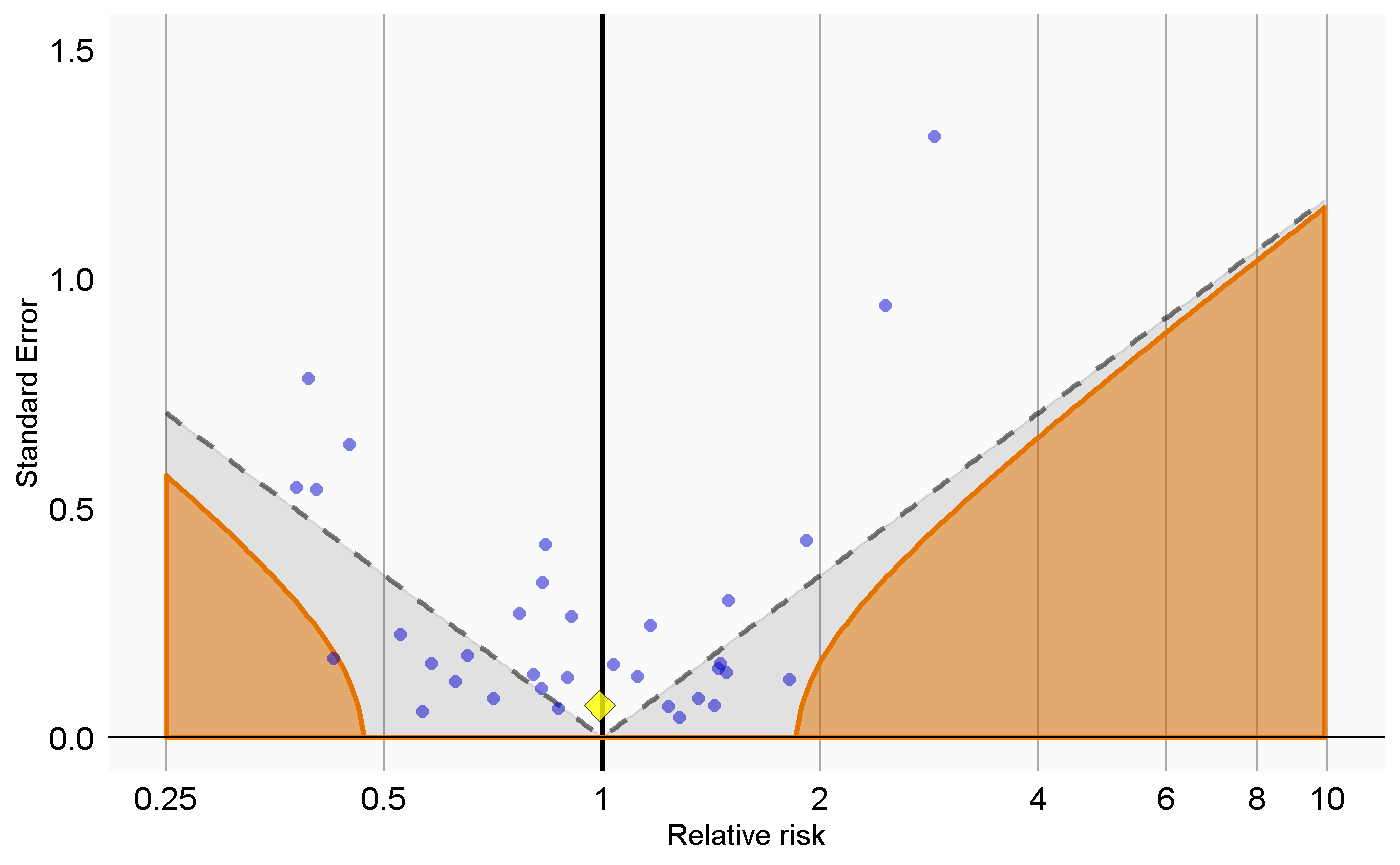
\includegraphics{../inst/doc/MultipleAnalyses_files/figure-latex/unnamed-chunk-17-1.pdf}

\begin{Shaded}
\begin{Highlighting}[]
\CommentTok{# Analysis 2: Matching}
\NormalTok{negCons <-}\StringTok{ }\NormalTok{analysisSum[analysisSum}\OperatorTok{$}\NormalTok{analysisId }\OperatorTok{==}\StringTok{ }\DecValTok{2} \OperatorTok{&}\StringTok{ }\NormalTok{analysisSum}\OperatorTok{$}\NormalTok{outcomeId }\OperatorTok{!=}\StringTok{ }\DecValTok{192671}\NormalTok{, ]}
\NormalTok{hoi <-}\StringTok{  }\NormalTok{analysisSum[analysisSum}\OperatorTok{$}\NormalTok{analysisId }\OperatorTok{==}\StringTok{ }\DecValTok{2} \OperatorTok{&}\StringTok{ }\NormalTok{analysisSum}\OperatorTok{$}\NormalTok{outcomeId }\OperatorTok{==}\StringTok{ }\DecValTok{192671}\NormalTok{, ]}
\NormalTok{null <-}\StringTok{ }\KeywordTok{fitNull}\NormalTok{(negCons}\OperatorTok{$}\NormalTok{logRr, negCons}\OperatorTok{$}\NormalTok{seLogRr)}
\KeywordTok{plotCalibrationEffect}\NormalTok{(negCons}\OperatorTok{$}\NormalTok{logRr, negCons}\OperatorTok{$}\NormalTok{seLogRr, hoi}\OperatorTok{$}\NormalTok{logRr, hoi}\OperatorTok{$}\NormalTok{seLogRr, null)}
\end{Highlighting}
\end{Shaded}

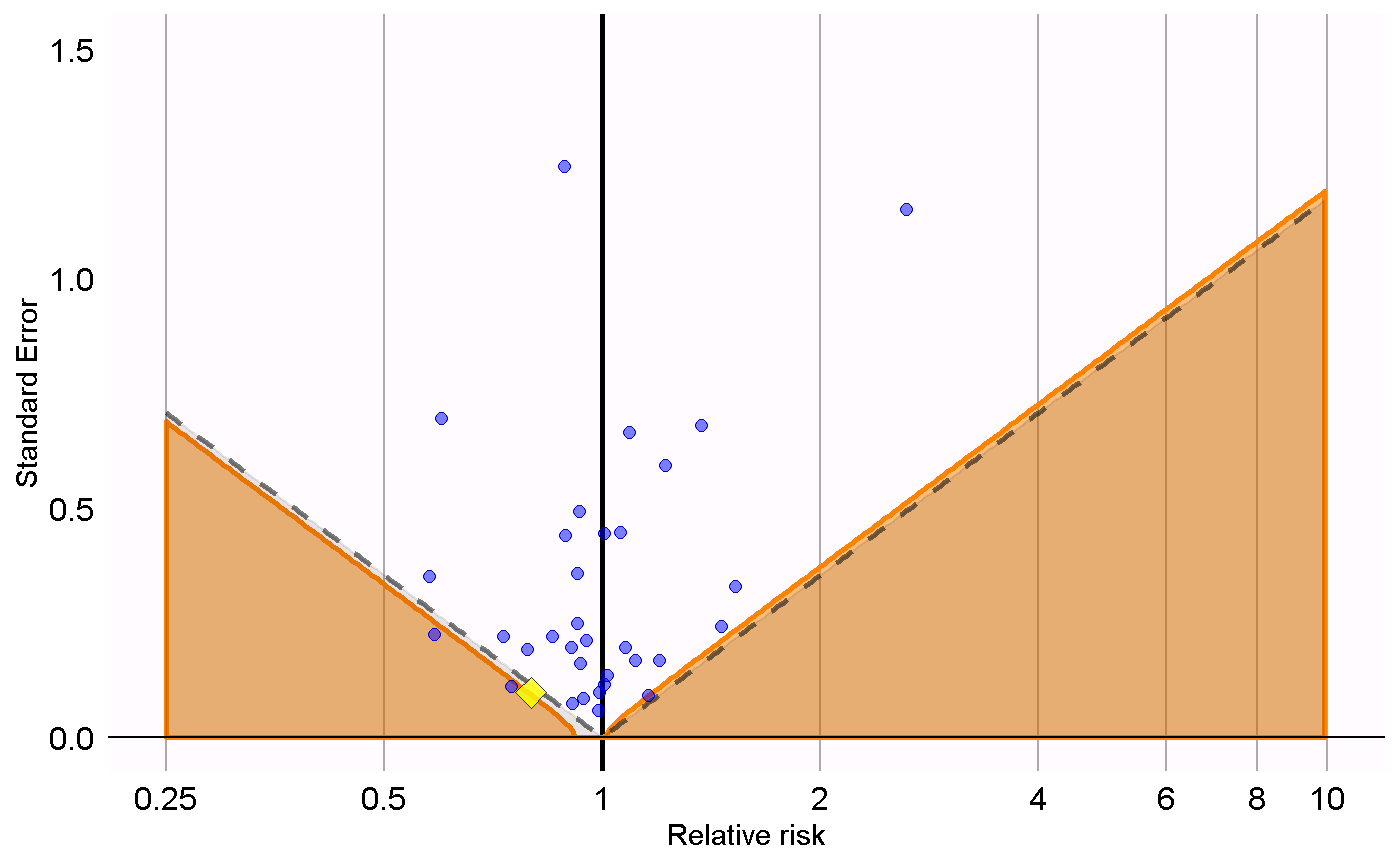
\includegraphics{../inst/doc/MultipleAnalyses_files/figure-latex/unnamed-chunk-19-1.pdf}

\begin{Shaded}
\begin{Highlighting}[]
\CommentTok{# Analysis 3: Stratification}
\NormalTok{negCons <-}\StringTok{ }\NormalTok{analysisSum[analysisSum}\OperatorTok{$}\NormalTok{analysisId }\OperatorTok{==}\StringTok{ }\DecValTok{3} \OperatorTok{&}\StringTok{ }\NormalTok{analysisSum}\OperatorTok{$}\NormalTok{outcomeId }\OperatorTok{!=}\StringTok{ }\DecValTok{192671}\NormalTok{, ]}
\NormalTok{hoi <-}\StringTok{  }\NormalTok{analysisSum[analysisSum}\OperatorTok{$}\NormalTok{analysisId }\OperatorTok{==}\StringTok{ }\DecValTok{3} \OperatorTok{&}\StringTok{ }\NormalTok{analysisSum}\OperatorTok{$}\NormalTok{outcomeId }\OperatorTok{==}\StringTok{ }\DecValTok{192671}\NormalTok{, ]}
\NormalTok{null <-}\StringTok{ }\KeywordTok{fitNull}\NormalTok{(negCons}\OperatorTok{$}\NormalTok{logRr, negCons}\OperatorTok{$}\NormalTok{seLogRr)}
\KeywordTok{plotCalibrationEffect}\NormalTok{(negCons}\OperatorTok{$}\NormalTok{logRr, negCons}\OperatorTok{$}\NormalTok{seLogRr, hoi}\OperatorTok{$}\NormalTok{logRr, hoi}\OperatorTok{$}\NormalTok{seLogRr, null)}
\end{Highlighting}
\end{Shaded}

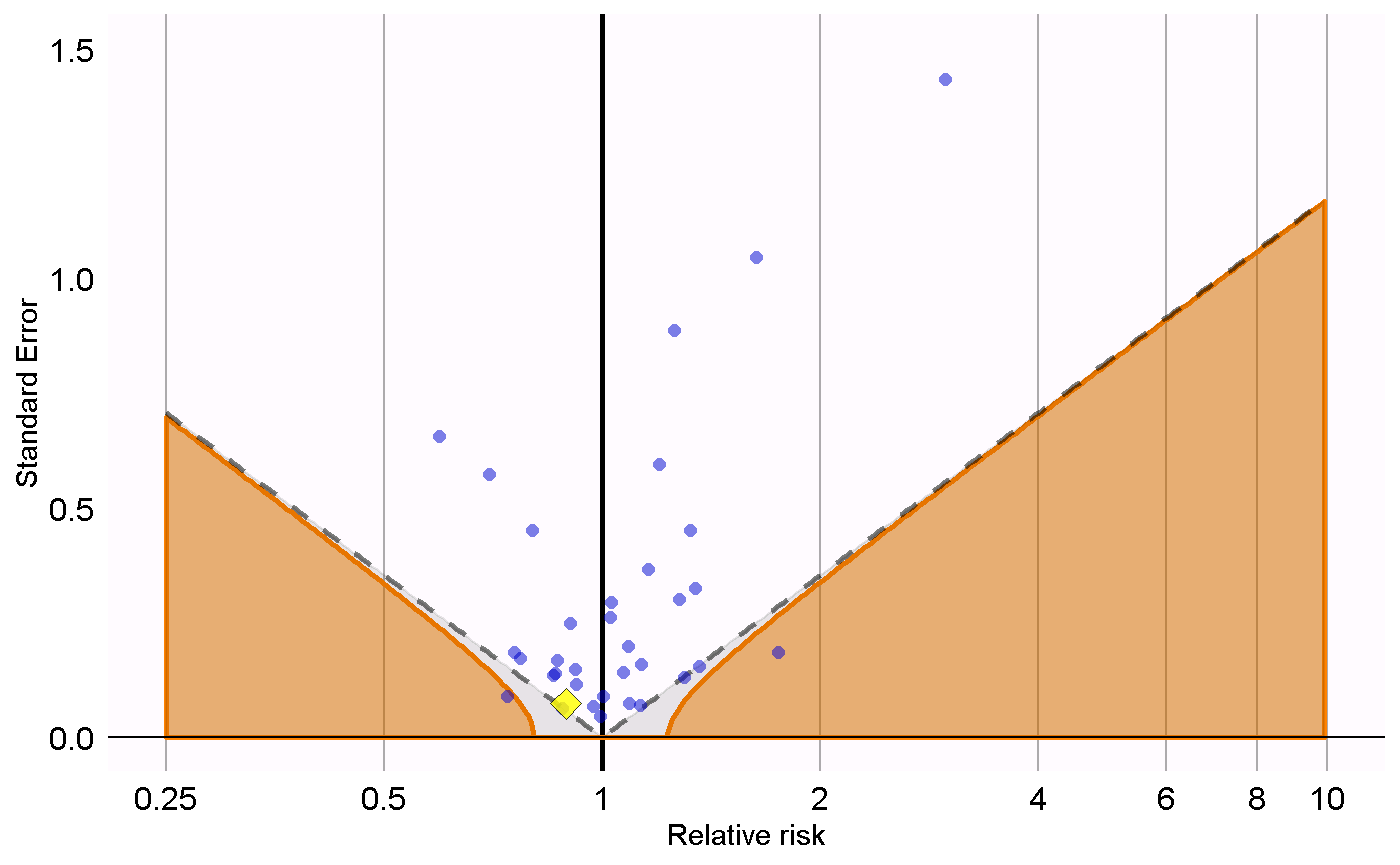
\includegraphics{../inst/doc/MultipleAnalyses_files/figure-latex/unnamed-chunk-21-1.pdf}

\begin{Shaded}
\begin{Highlighting}[]
\CommentTok{# Analysis 4: Inverse probability of treatment weighting}
\NormalTok{negCons <-}\StringTok{ }\NormalTok{analysisSum[analysisSum}\OperatorTok{$}\NormalTok{analysisId }\OperatorTok{==}\StringTok{ }\DecValTok{4} \OperatorTok{&}\StringTok{ }\NormalTok{analysisSum}\OperatorTok{$}\NormalTok{outcomeId }\OperatorTok{!=}\StringTok{ }\DecValTok{192671}\NormalTok{, ]}
\NormalTok{hoi <-}\StringTok{  }\NormalTok{analysisSum[analysisSum}\OperatorTok{$}\NormalTok{analysisId }\OperatorTok{==}\StringTok{ }\DecValTok{4} \OperatorTok{&}\StringTok{ }\NormalTok{analysisSum}\OperatorTok{$}\NormalTok{outcomeId }\OperatorTok{==}\StringTok{ }\DecValTok{192671}\NormalTok{, ]}
\NormalTok{null <-}\StringTok{ }\KeywordTok{fitNull}\NormalTok{(negCons}\OperatorTok{$}\NormalTok{logRr, negCons}\OperatorTok{$}\NormalTok{seLogRr)}
\KeywordTok{plotCalibrationEffect}\NormalTok{(negCons}\OperatorTok{$}\NormalTok{logRr, negCons}\OperatorTok{$}\NormalTok{seLogRr, hoi}\OperatorTok{$}\NormalTok{logRr, hoi}\OperatorTok{$}\NormalTok{seLogRr, null)}
\end{Highlighting}
\end{Shaded}

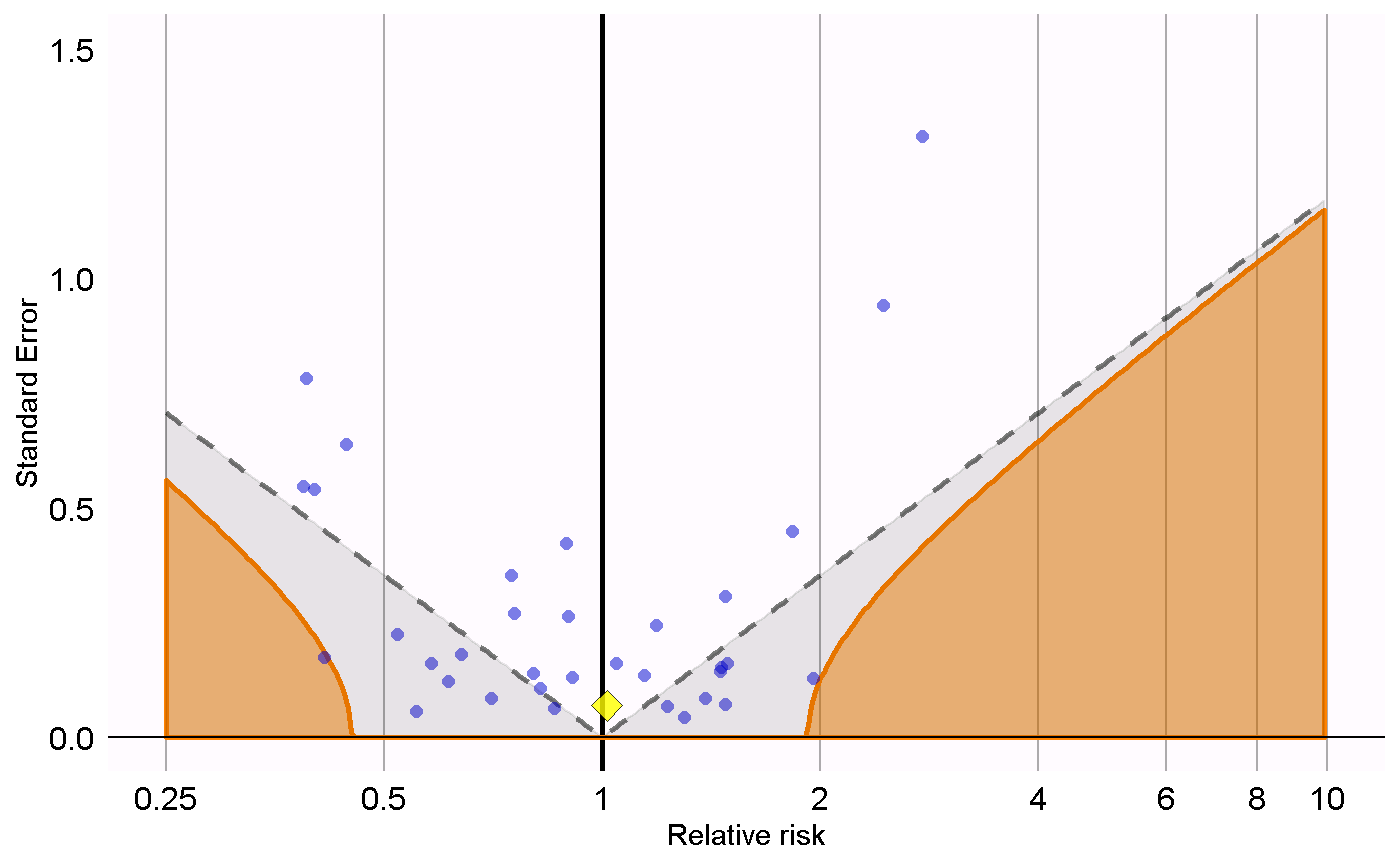
\includegraphics{../inst/doc/MultipleAnalyses_files/figure-latex/unnamed-chunk-23-1.pdf}

\begin{Shaded}
\begin{Highlighting}[]
\CommentTok{# Analysis 5: Stratification plus full outcome model}
\NormalTok{negCons <-}\StringTok{ }\NormalTok{analysisSum[analysisSum}\OperatorTok{$}\NormalTok{analysisId }\OperatorTok{==}\StringTok{ }\DecValTok{5} \OperatorTok{&}\StringTok{ }\NormalTok{analysisSum}\OperatorTok{$}\NormalTok{outcomeId }\OperatorTok{!=}\StringTok{ }\DecValTok{192671}\NormalTok{, ]}
\NormalTok{hoi <-}\StringTok{  }\NormalTok{analysisSum[analysisSum}\OperatorTok{$}\NormalTok{analysisId }\OperatorTok{==}\StringTok{ }\DecValTok{5} \OperatorTok{&}\StringTok{ }\NormalTok{analysisSum}\OperatorTok{$}\NormalTok{outcomeId }\OperatorTok{==}\StringTok{ }\DecValTok{192671}\NormalTok{, ]}
\NormalTok{null <-}\StringTok{ }\KeywordTok{fitNull}\NormalTok{(negCons}\OperatorTok{$}\NormalTok{logRr, negCons}\OperatorTok{$}\NormalTok{seLogRr)}
\KeywordTok{plotCalibrationEffect}\NormalTok{(negCons}\OperatorTok{$}\NormalTok{logRr, negCons}\OperatorTok{$}\NormalTok{seLogRr, hoi}\OperatorTok{$}\NormalTok{logRr, hoi}\OperatorTok{$}\NormalTok{seLogRr, null)}
\end{Highlighting}
\end{Shaded}

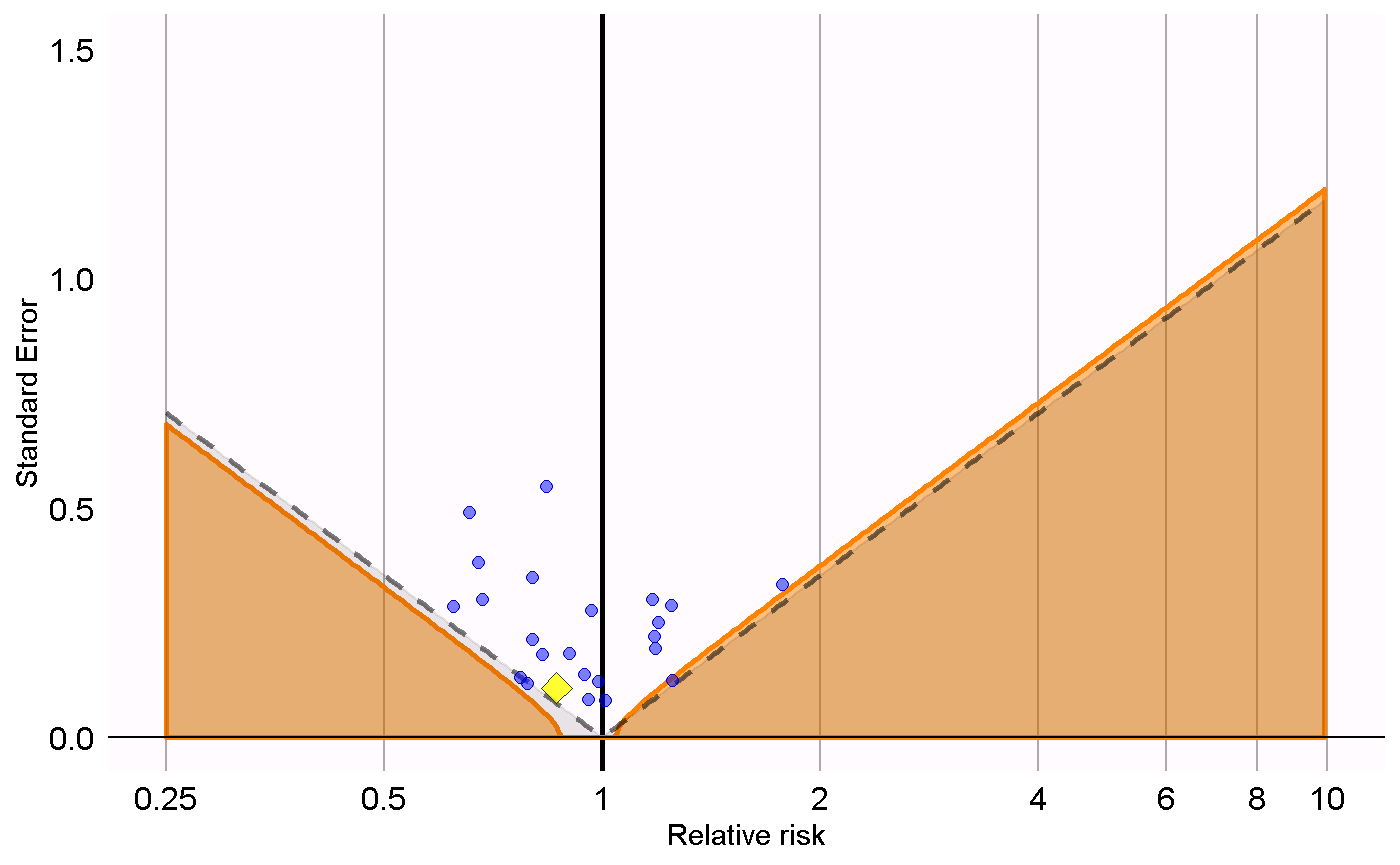
\includegraphics{../inst/doc/MultipleAnalyses_files/figure-latex/unnamed-chunk-25-1.pdf}

Analysis 6 explored interactions with certain variables. The estimates
for these interaction terms are also stored in the analysis summary. We
can examine whether these estimates are also consistent with the null.
In this example we consider the interaction with `gender = female'
(covariate ID 8532001):

\begin{Shaded}
\begin{Highlighting}[]
\CommentTok{# Analysis 6: Stratification plus interaction terms}
\NormalTok{negCons <-}\StringTok{ }\NormalTok{analysisSum[analysisSum}\OperatorTok{$}\NormalTok{analysisId }\OperatorTok{==}\StringTok{ }\DecValTok{6} \OperatorTok{&}\StringTok{ }\NormalTok{analysisSum}\OperatorTok{$}\NormalTok{outcomeId }\OperatorTok{!=}\StringTok{ }\DecValTok{192671}\NormalTok{, ]}
\NormalTok{hoi <-}\StringTok{  }\NormalTok{analysisSum[analysisSum}\OperatorTok{$}\NormalTok{analysisId }\OperatorTok{==}\StringTok{ }\DecValTok{6} \OperatorTok{&}\StringTok{ }\NormalTok{analysisSum}\OperatorTok{$}\NormalTok{outcomeId }\OperatorTok{==}\StringTok{ }\DecValTok{192671}\NormalTok{, ]}
\NormalTok{null <-}\StringTok{ }\KeywordTok{fitNull}\NormalTok{(negCons}\OperatorTok{$}\NormalTok{logRrI8532001, negCons}\OperatorTok{$}\NormalTok{seLogRrI8532001)}
\KeywordTok{plotCalibrationEffect}\NormalTok{(}\DataTypeTok{logRrNegatives =}\NormalTok{ negCons}\OperatorTok{$}\NormalTok{logRrI8532001, }
                      \DataTypeTok{seLogRrNegatives =}\NormalTok{ negCons}\OperatorTok{$}\NormalTok{seLogRrI8532001, }
                      \DataTypeTok{logRrPositives =}\NormalTok{ hoi}\OperatorTok{$}\NormalTok{logRrI8532001, }
                      \DataTypeTok{seLogRrPositives =}\NormalTok{ hoi}\OperatorTok{$}\NormalTok{seLogRrI8532001, null)}
\end{Highlighting}
\end{Shaded}

\begin{verbatim}
## Warning in fitNull(negCons$logRrI8532001, negCons$seLogRrI8532001): Estimate(s) with NA standard error detected. Removing before fitting null distribution
\end{verbatim}

\begin{verbatim}
## Warning: Removed 9 rows containing missing values (geom_point).
\end{verbatim}

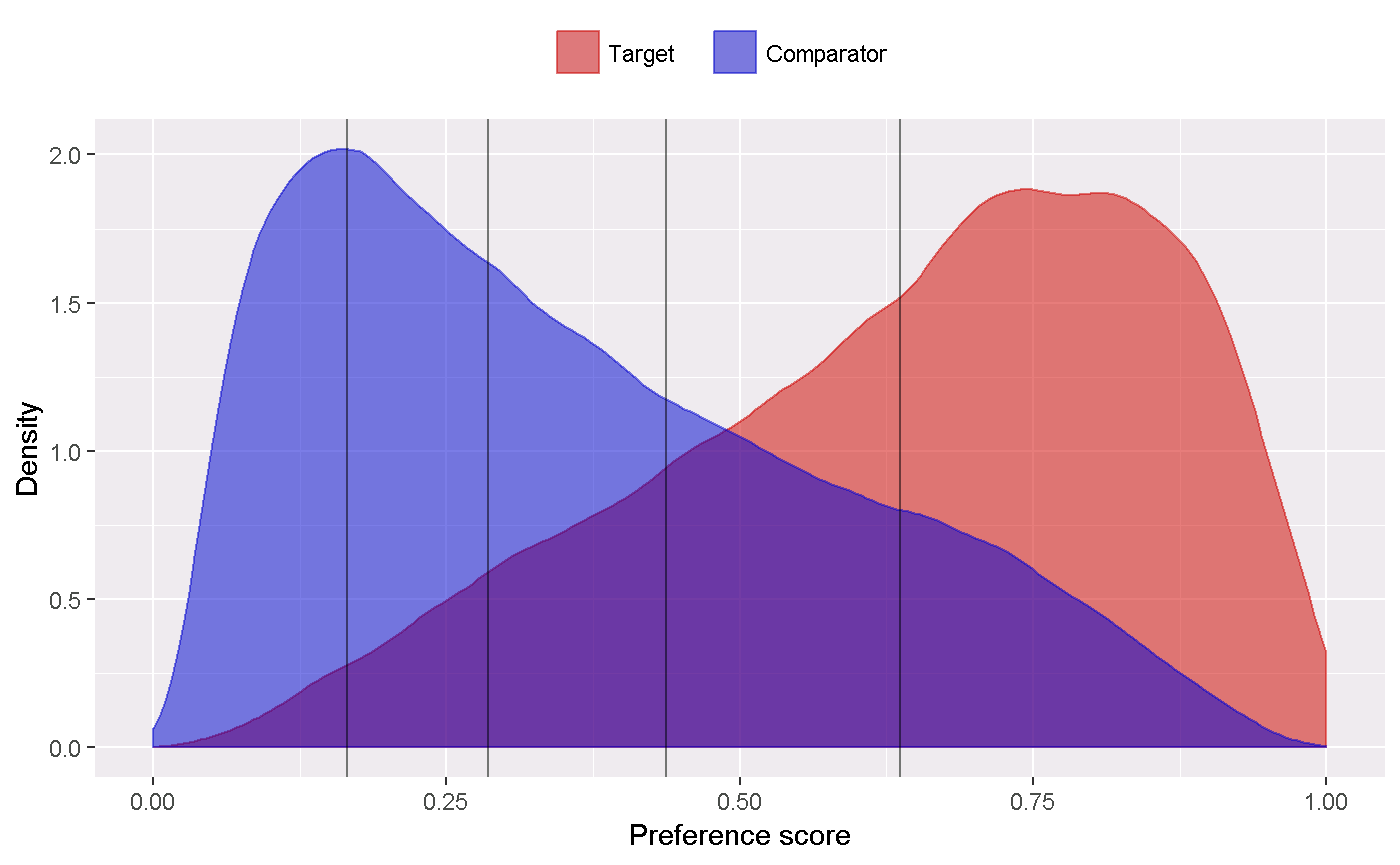
\includegraphics{../inst/doc/MultipleAnalyses_files/figure-latex/unnamed-chunk-27-1.pdf}

\hypertarget{acknowledgments}{%
\section{Acknowledgments}\label{acknowledgments}}

Considerable work has been dedicated to provide the
\texttt{CohortMethod} package.

\begin{Shaded}
\begin{Highlighting}[]
\KeywordTok{citation}\NormalTok{(}\StringTok{"CohortMethod"}\NormalTok{)}
\end{Highlighting}
\end{Shaded}

\begin{verbatim}
## 
## To cite package 'CohortMethod' in publications use:
## 
##   Martijn Schuemie, Marc Suchard and Patrick Ryan (2020). CohortMethod: New-user cohort method with large scale propensity and outcome models.
##   https://ohdsi.github.io/CohortMethod, https://github.com/OHDSI/CohortMethod.
## 
## A BibTeX entry for LaTeX users is
## 
##   @Manual{,
##     title = {CohortMethod: New-user cohort method with large scale propensity and outcome models},
##     author = {Martijn Schuemie and Marc Suchard and Patrick Ryan},
##     year = {2020},
##     note = {https://ohdsi.github.io/CohortMethod, https://github.com/OHDSI/CohortMethod},
##   }
\end{verbatim}

Further, \texttt{CohortMethod} makes extensive use of the
\texttt{Cyclops} package.

\begin{Shaded}
\begin{Highlighting}[]
\KeywordTok{citation}\NormalTok{(}\StringTok{"Cyclops"}\NormalTok{)}
\end{Highlighting}
\end{Shaded}

\begin{verbatim}
## 
## To cite Cyclops in publications use:
## 
## Suchard MA, Simpson SE, Zorych I, Ryan P, Madigan D (2013). "Massive parallelization of serial inference algorithms for complex generalized linear
## models." _ACM Transactions on Modeling and Computer Simulation_, *23*, 10. <URL: http://dl.acm.org/citation.cfm?id=2414791>.
## 
## A BibTeX entry for LaTeX users is
## 
##   @Article{,
##     author = {M. A. Suchard and S. E. Simpson and I. Zorych and P. Ryan and D. Madigan},
##     title = {Massive parallelization of serial inference algorithms for complex generalized linear models},
##     journal = {ACM Transactions on Modeling and Computer Simulation},
##     volume = {23},
##     pages = {10},
##     year = {2013},
##     url = {http://dl.acm.org/citation.cfm?id=2414791},
##   }
\end{verbatim}

This work is supported in part through the National Science Foundation
grant IIS 1251151.

\end{document}
